\documentclass[aspectratio=169]{beamer}
\usetheme{Madrid}
\usecolortheme{seahorse}
\usepackage{amsmath, amssymb}
\usepackage{booktabs}
\usepackage{multirow}
\usepackage{tikz}
\usetikzlibrary{arrows.meta, shapes.geometric, positioning, fit, backgrounds}
\usepackage{xcolor}

% Custom colors
\definecolor{navyblue}{RGB}{13, 27, 42}
\definecolor{teal}{RGB}{13, 148, 136}
\definecolor{lightmint}{RGB}{204, 251, 241}
\definecolor{amber}{RGB}{245, 158, 11}
\definecolor{slategray}{RGB}{100, 116, 139}

\setbeamercolor{palette primary}{bg=navyblue, fg=white}
\setbeamercolor{palette secondary}{bg=teal, fg=white}
\setbeamercolor{palette tertiary}{bg=navyblue, fg=white}
\setbeamercolor{palette quaternary}{bg=navyblue, fg=white}
\setbeamercolor{structure}{fg=teal}
\setbeamercolor{section in toc}{fg=navyblue}
\setbeamercolor{alerted text}{fg=amber}
\setbeamercolor{block title}{bg=teal, fg=white}
\setbeamercolor{block body}{bg=lightmint, fg=black}
\setbeamercolor{frametitle}{bg=navyblue, fg=white}
\setbeamerfont{frametitle}{series=\bfseries}
\setbeamertemplate{navigation symbols}{}

\title[Aleatoric GSL for ADMET Curation]{\textbf{Evidential Graph Structure Learning}\\[4pt]for Automated Dataset Curation in ADMET Prediction}
\author[Shukla \& Tripathy]{%
\begin{tabular}{cc}
Inesh Shukla & Arihant Tripathy \\[2pt]
{\small\texttt{2023113008}} & {\small\texttt{2023111026}}
\end{tabular}}
\institute[IIIT Hyderabad]{International Institute of Information Technology, Hyderabad\\Machine Learning for Natural Sciences (MLNS)}
\date{Spring 2026}

\begin{document}

% ─────────────────────────────────────────────
% SLIDE 1: Title
% ─────────────────────────────────────────────
\begin{frame}
\titlepage
\end{frame}

% ─────────────────────────────────────────────
% SLIDE 2: Outline
% ─────────────────────────────────────────────
\begin{frame}{Outline}
\tableofcontents
\end{frame}

% ─────────────────────────────────────────────
\section{Problem Statement}
% ─────────────────────────────────────────────

% ─────────────────────────────────────────────
% SLIDE 3: The Core Problem
% ─────────────────────────────────────────────
\begin{frame}[t]{The Core Problem: Noisy ADMET Benchmarks}
\begin{columns}[T]
\begin{column}{0.48\textwidth}
\begin{block}{Biological Assay Variability}
Public ADMET datasets (e.g.\ \textbf{TDC Caco-2}) are treated as ground truth, yet inter-laboratory variability introduces \alert{severe, unrecorded label noise}:
\begin{itemize}
    \item pH, incubation time, cell passage number
    \item Same compound measured under different protocols
    \item Noise \textbf{indistinguishable} from the true signal
\end{itemize}
\end{block}
\end{column}
\begin{column}{0.48\textwidth}
\begin{block}{Downstream Effect}
Standard objectives minimize loss under the \emph{corrupted} distribution $\Rightarrow$ \alert{systematic bias against robust predictors}.
\end{block}
\vspace{6pt}
\begin{center}
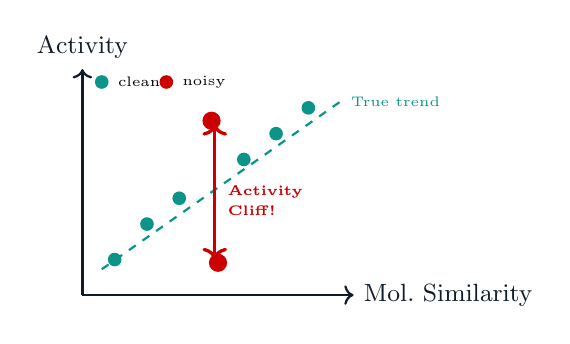
\begin{tikzpicture}[scale=0.82]
  \draw[->, thick, color=navyblue] (0,0) -- (4.2,0) node[right, font=\small] {Mol.\ Similarity};
  \draw[->, thick, color=navyblue] (0,0) -- (0,3.5) node[above, font=\small] {Activity};
  \draw[-, thick, color=teal, dashed] (0.3,0.4) -- (4.0,3.0) node[right, font=\tiny, color=teal] {True trend};
  \foreach \x/\y in {0.5/0.55, 1.0/1.1, 1.5/1.5, 2.5/2.1, 3.0/2.5, 3.5/2.9}{
    \fill[teal] (\x,\y) circle (3pt);
  }
  \fill[red!80!black] (2.0,2.7) circle (4pt);
  \fill[red!80!black] (2.1,0.5) circle (4pt);
  \draw[<->, red!80!black, very thick] (2.05,0.55) -- (2.05,2.65);
  \node[font=\tiny, color=red!80!black, right] at (2.1,1.6) {\textbf{Activity}};
  \node[font=\tiny, color=red!80!black, right] at (2.1,1.3) {\textbf{Cliff!}};
  \fill[teal] (0.3,3.3) circle (3pt); \node[font=\tiny, right] at (0.4,3.3) {clean};
  \fill[red!80!black] (1.3,3.3) circle (3pt); \node[font=\tiny, right] at (1.4,3.3) {noisy};
\end{tikzpicture}
\end{center}
\end{column}
\end{columns}
\end{frame}

% ─────────────────────────────────────────────
% SLIDE 4: Why GNNs Make It Worse
% ─────────────────────────────────────────────
\begin{frame}[shrink=5]{Why Standard GNNs Amplify the Problem}
\begin{center}
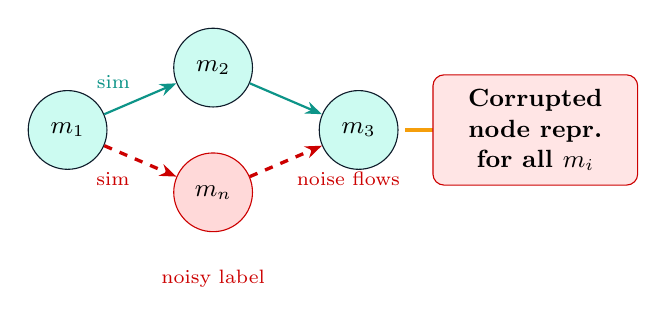
\begin{tikzpicture}[
  scale=0.66,
  node distance=1.8cm,
  mol/.style={circle, draw=navyblue, fill=lightmint, minimum size=1.0cm, font=\small\bfseries},
  noisymol/.style={circle, draw=red!80!black, fill=red!15, minimum size=1.0cm, font=\small\bfseries},
  arr/.style={-{Stealth[length=6pt]}, thick}
]
  \node[mol] (A) at (0,0)    {$m_1$};
  \node[mol] (B) at (2.8,1.2)  {$m_2$};
  \node[noisymol] (N) at (2.8,-1.2) {$m_n$};
  \node[mol] (C) at (5.6,0)  {$m_3$};

  \draw[arr, color=teal] (A) -- (B) node[midway, above left, font=\scriptsize] {sim};
  \draw[arr, color=red!80!black, dashed, very thick] (A) -- (N)
      node[midway, below left, font=\scriptsize, color=red!80!black] {sim};
  \draw[arr, color=teal] (B) -- (C);
  \draw[arr, color=red!80!black, dashed, very thick] (N) -- (C)
      node[midway, below right, font=\scriptsize, color=red!80!black] {noise flows};

  \node[font=\scriptsize, color=red!80!black, below=0.35cm of N] {noisy label};
  \draw[-{Stealth[length=8pt]}, ultra thick, color=amber] (6.5,0) -- (7.5,0);
  \node[draw=red!80!black, fill=red!10, rounded corners, font=\small, align=center,
        minimum width=2.6cm, minimum height=1.4cm] at (9.0,0)
      {\textbf{Corrupted}\\\textbf{node repr.}\\\textbf{for all $m_i$}};
\end{tikzpicture}
\end{center}
\vspace{2pt}
\begin{columns}[T]
\begin{column}{0.48\textwidth}
\begin{alertblock}{The Smear Effect}
GNN message-passing \textbf{aggregates noise} from structurally similar neighbors. At activity cliffs, one bad label degrades the representation of every nearby molecule.
\end{alertblock}
\end{column}
\begin{column}{0.48\textwidth}
\begin{block}{Empirical Confirmation (Phase 1B)}
Our baseline GSL model achieved \textbf{MAE = 0.4589} — \alert{worse than} the plain MLP baseline (MAE = 0.3711), directly confirming noise propagation in practice.
\end{block}
\end{column}
\end{columns}
\end{frame}

% ─────────────────────────────────────────────
% SLIDE 5: Research Questions
% ─────────────────────────────────────────────
\begin{frame}{Research Questions \& Objectives}
\begin{center}
\large\color{navyblue}
\textit{``Can a model learn \textbf{which data to trust} and use that knowledge\\
to clean the dataset it was trained on?''}
\end{center}
\vspace{10pt}
\begin{columns}[T]
\begin{column}{0.3\textwidth}
\begin{block}{\centering \textbf{RQ 1}}
\centering Can graph structure learning, augmented with evidential uncertainty, \textbf{detect noisy labels} at activity cliffs?
\end{block}
\end{column}
\begin{column}{0.3\textwidth}
\begin{block}{\centering \textbf{RQ 2}}
\centering Can the estimated \textbf{aleatoric uncertainty} gate message passing to prevent noise propagation?
\end{block}
\end{column}
\begin{column}{0.3\textwidth}
\begin{block}{\centering \textbf{RQ 3}}
\centering Does \textbf{removing/down-weighting} flagged molecules improve downstream baseline models?
\end{block}
\end{column}
\end{columns}
\vspace{10pt}
\begin{center}
\textbf{Datasets:} TDC Caco-2 Wang ($N=637$) \quad \textbullet \quad TDC Lipophilicity AstraZeneca ($N{\approx}4{,}200$)\\[2pt]
\textbf{Embeddings:} Frozen MolFormer-XL (768-d) as node features
\end{center}
\end{frame}

% ─────────────────────────────────────────────
\section{Proposed Solution \& Architecture}
% ─────────────────────────────────────────────

% ─────────────────────────────────────────────
% SLIDE 6: Architecture Overview
% ─────────────────────────────────────────────
\begin{frame}{Proposed Architecture: Evidential GSL}
\begin{center}
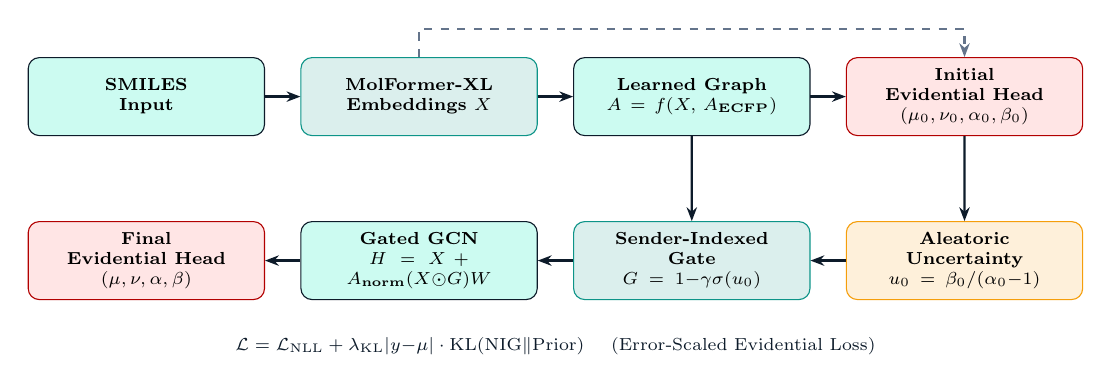
\begin{tikzpicture}[
  node distance=1.2cm and 0.5cm,
  box/.style={draw=navyblue, fill=lightmint, rounded corners=4pt,
              minimum height=1.1cm, text width=3.1cm,
              font=\scriptsize\bfseries, align=center},
  redbox/.style={draw=red!70!black, fill=red!10, rounded corners=4pt,
                 minimum height=1.1cm, text width=3.1cm,
                 font=\scriptsize\bfseries, align=center},
  tealbox/.style={draw=teal, fill=teal!15, rounded corners=4pt,
                  minimum height=1.1cm, text width=3.1cm,
                  font=\scriptsize\bfseries, align=center},
  amberbox/.style={draw=amber, fill=amber!15, rounded corners=4pt,
                   minimum height=1.1cm, text width=3.1cm,
                   font=\scriptsize\bfseries, align=center},
  arr/.style={-{Stealth[length=5pt]}, thick, color=navyblue},
  scale=0.9, transform shape
]
  \node[box]     (mol)  {SMILES\\Input};
  \node[tealbox] (emb)  [right=of mol] {MolFormer-XL\\Embeddings $X$};
  \node[box]     (gsl)  [right=of emb] {Learned Graph\\$A = f(X,\,A_\text{ECFP})$};
  \node[redbox]  (init) [right=of gsl] {Initial\\Evidential Head\\$(\mu_0,\nu_0,\alpha_0,\beta_0)$};

  \node[redbox]   (final)[below=of mol]  {Final\\Evidential Head\\$(\mu,\nu,\alpha,\beta)$};
  \node[box]      (gcn)  [below=of emb]  {Gated GCN\\$H=X+A_\text{norm}(X{\odot}G)W$};
  \node[tealbox]  (gate) [below=of gsl]  {Sender-Indexed\\Gate\\$G = 1{-}\gamma\sigma(u_0)$};
  \node[amberbox] (u0)   [below=of init] {Aleatoric\\Uncertainty\\$u_0=\beta_0/(\alpha_0{-}1)$};

  \draw[arr] (mol.east)  -- (emb.west);
  \draw[arr] (emb.east)  -- (gsl.west);
  \draw[arr] (gsl.east)  -- (init.west);
  \draw[arr, dashed, color=slategray] (emb.north) -- ++(0, 0.4) -| (init.north);
  \draw[arr] (init.south) -- (u0.north);
  \draw[arr] (gsl.south)  -- (gate.north);
  \draw[arr] (u0.west)   -- (gate.east);
  \draw[arr] (gate.west) -- (gcn.east);
  \draw[arr] (gcn.west)  -- (final.east);

  \path (final.south) -- (u0.south) node[midway, below=0.4cm, font=\scriptsize, color=navyblue, align=center]
    {$\mathcal{L}=\mathcal{L}_\text{NLL}
      +\lambda_\text{KL}|y{-}\mu|\cdot\text{KL}(\text{NIG}\|\text{Prior})$
     \quad (Error-Scaled Evidential Loss)};
\end{tikzpicture}
\end{center}
\vspace{2pt}
\begin{columns}[T]
\begin{column}{0.48\textwidth}
{\small \textbf{Key innovation:} aleatoric uncertainty $u_j$ from a
\emph{sender} suppresses its contribution to all neighbors ---
preventing noise at activity cliffs from poisoning nearby embeddings.}
\end{column}
\begin{column}{0.48\textwidth}
{\small \textbf{Skip connection} ensures a noisy node's own
representation is not zeroed by its own gate ---
isolating self-update from neighbor aggregation.}
\end{column}
\end{columns}
\end{frame}

% ─────────────────────────────────────────────
% SLIDE 7: Filter-and-Retrain Protocol
% ─────────────────────────────────────────────
\begin{frame}[t]{The Filter-and-Retrain \& Soft-Weighting Protocols}
\begin{columns}[T]
\begin{column}{0.48\textwidth}
\textbf{Protocol A — Hard Filtering (Phase 3A/3B)}
\vspace{1pt}
\begin{center}
\begin{tikzpicture}[
  step/.style={draw=navyblue, fill=lightmint, rounded corners,
               font=\scriptsize, minimum width=3.0cm, minimum height=0.45cm,
               align=center},
  arr/.style={-{Stealth[length=5pt]}, thick, color=teal}
]
  \node[step] (s1) at (0,0)     {Train Evidential GSL};
  \node[step] (s2) at (0,-0.75) {Compute $u_i$ for all molecules};
  \node[step, draw=red!70!black, fill=red!10]   (s3) at (0,-1.50) {Remove top-$k$\% ($u > \tau$)};
  \node[step, draw=teal,         fill=teal!15]  (s4) at (0,-2.25) {Retrain Baseline MLP};
  \node[step, draw=amber,        fill=amber!15] (s5) at (0,-3.00) {Evaluate Generalization};
  
  \draw[arr] (s1)--(s2); \draw[arr] (s2)--(s3);
  \draw[arr] (s3)--(s4); \draw[arr] (s4)--(s5);
\end{tikzpicture}
\vspace{1pt}
\begin{block}{Motivation}
\small Hard filtering on a small dataset (Caco-2, $N{=}637$) causes \alert{data starvation} — soft weighting is safer.
\end{block}
\end{center}
\end{column}
\begin{column}{0.48\textwidth}
\textbf{Protocol B — Soft Weighting (Phase 3C)}
\vspace{4pt}\\
Instead of deleting molecules, \emph{down-weight} their contribution:
\[
\mathcal{L} = \frac{1}{N}\sum_i \underbrace{e^{-\gamma u_i}}_{\text{weight}} \cdot (\hat{y}_i - y_i)^2
\]
\begin{itemize}\small
  \item $\gamma = 0$: standard MSE (baseline)
  \item $\gamma > 0$: noisy molecules contribute less
  \item Preserves full chemical diversity
\end{itemize}
\end{column}
\end{columns}
\end{frame}

% ─────────────────────────────────────────────
\section{Results}
% ─────────────────────────────────────────────

% ─────────────────────────────────────────────
% SLIDE 8: Architectural Contribution — GSL to Evidential GSL Across Datasets
% ─────────────────────────────────────────────
\begin{frame}[t]{Architectural Contribution: GSL $\to$ Evidential GSL}
\begin{center}
\footnotesize
\setlength{\tabcolsep}{5pt}
\begin{tabular}{llccc}
\toprule
\textbf{Dataset} & \textbf{Model} & \textbf{MAE} & \textbf{RMSE} & \textbf{Outcome} \\
\midrule
\multirow{2}{*}{\textbf{Caco-2} ($N{=}637$)}
  & Simple GSL        & 0.4589 & 0.5567 & \textcolor{red!70!black}{Fail: noise propagation} \\
  & \textbf{Evidential GSL} & \textbf{0.3777} & \textbf{0.4615} & \textcolor{teal}{\textbf{Recovers ($-16.4\%$)}} \\
\midrule
\multirow{2}{*}{\textbf{Lipo} ($N{=}4{,}200$)}
  & Simple GSL        & 0.7630 & 0.8101 & \textcolor{red!70!black}{Degrades vs.\ MLP} \\
  & \textbf{Evidential GSL} & \textbf{0.6090} & \textbf{0.7777} & \textcolor{teal}{\textbf{Best single model ($-0.7\%$)}} \\
\midrule
\multirow{2}{*}{\textbf{AqSolDB} ($N{=}9{,}982$)}
  & Simple GSL        & 1.2543 & 1.6344 & \textcolor{red!70!black}{Fails for same reason} \\
  & \textbf{Evidential GSL} & \textbf{0.9091} & \textbf{1.2139} & \textcolor{teal}{\textbf{Recovers to MLP level ($-27.5\%$)}} \\
\bottomrule
\end{tabular}
\end{center}
\vspace{6pt}
\begin{columns}[T]
\begin{column}{0.55\textwidth}
\begin{alertblock}{Consistent Pattern Across All Three Datasets}
\footnotesize \textbf{Simple GSL always degrades} — noise propagation is universal. \textbf{Evidential GSL consistently recovers} by gating message passing with aleatoric uncertainty.
\end{alertblock}
\end{column}
\begin{column}{0.42\textwidth}
\begin{block}{Key Takeaway}
\footnotesize The transition GSL $\to$ Evidential GSL is \textbf{strictly necessary}: without evidential gating, graph structure learning is harmful. Our fix is \emph{dataset-agnostic}.
\end{block}
\end{column}
\end{columns}
\end{frame}

% ─────────────────────────────────────────────
% SLIDE 9: Lipophilicity Full Results
% ─────────────────────────────────────────────
\begin{frame}[t,shrink=15]{Lipophilicity Results: Soft-Weighting Sweep}
\textbf{Dataset:} TDC Lipophilicity AstraZeneca ($N{=}2{,}940$ train) \quad 10 seeds per $\gamma$
\vspace{2pt}
\begin{columns}[T]
\begin{column}{0.60\textwidth}
\begin{block}{MAE by Base Model and $\gamma$}
\centering\footnotesize
\renewcommand{\arraystretch}{0.85}
\setlength{\tabcolsep}{3pt}
\begin{tabular}{lcccc}
\toprule
\textbf{Model} & $\gamma{=}0$ & Best $\gamma$ & \textbf{Best MAE} & $\Delta$ \\
\midrule
MLP (MolFormer) & $0.6134{\pm}0.0145$ & 20.0 & $\mathbf{0.6040{\pm}0.0111}$ & \textcolor{teal}{$-1.5\%$} \\
AttentiveFP     & $0.6157{\pm}0.0116$ & 15.0 & $\mathbf{0.5999{\pm}0.0137}$ & \textcolor{teal}{$-2.6\%$} \\
GCN (Evid.~GSL) & $0.7630{\pm}0.1026$ & 12.5 & $0.7094{\pm}0.0812$ & \textcolor{teal}{$-7.0\%$} \\
\bottomrule
\end{tabular}
\end{block}
\begin{block}{MLP $\gamma$ Sweep Detail}
\centering\scriptsize
\renewcommand{\arraystretch}{0.85}
\setlength{\tabcolsep}{3pt}
\begin{tabular}{ccccc}
\toprule
$\gamma$ & MAE & RMSE & $r$ & $\rho$ \\
\midrule
0.0  & $0.6134{\pm}0.0145$ & $0.7849{\pm}0.0159$ & $0.756$ & $0.731$ \\
7.0  & $0.6069{\pm}0.0077$ & $0.7758{\pm}0.0077$ & $0.760$ & $0.737$ \\
10.0 & $0.6060{\pm}0.0070$ & $0.7760{\pm}0.0061$ & $0.760$ & $0.738$ \\
12.5 & $0.6052{\pm}0.0147$ & $0.7747{\pm}0.0150$ & $0.760$ & $0.740$ \\
15.0 & $0.6054{\pm}0.0130$ & $0.7758{\pm}0.0150$ & $0.761$ & $0.742$ \\
\textbf{20.0} & $\mathbf{0.6040{\pm}0.0111}$ & $\mathbf{0.7739{\pm}0.0126}$ & $\mathbf{0.760}$ & $\mathbf{0.744}$ \\
\bottomrule
\end{tabular}
\end{block}
\end{column}
\begin{column}{0.37\textwidth}
\begin{alertblock}{Key Findings}
\footnotesize
\begin{itemize}
  \item Soft-weighting improves \textbf{all three} base models
  \item Monotonic improvement up to $\gamma{=}20$ for MLP
  \item Large $N$ $\Rightarrow$ denser uncertainty scores $\Rightarrow$ higher optimal $\gamma$ (12.5--20) vs.\ Caco-2 (2.0)
\end{itemize}
\end{alertblock}
\vspace{4pt}
\begin{block}{Curation Principle}
\footnotesize Uncertainty ranks should be used as \emph{weights}, not hard removal rules. Dataset noise is relative to the feature representation.
\end{block}
\end{column}
\end{columns}
\end{frame}

% ─────────────────────────────────────────────
% SLIDE 10: Caco-2 Full Results
% ─────────────────────────────────────────────
\begin{frame}[t,shrink=15]{Caco-2 Results: Soft-Weighting Sweep}
\textbf{Dataset:} TDC Caco-2 Wang ($N{=}637$) \quad 10 seeds per $\gamma$
\vspace{2pt}
\begin{columns}[T]
\begin{column}{0.60\textwidth}
\begin{block}{MAE by Base Model and $\gamma$}
\centering\footnotesize
\renewcommand{\arraystretch}{0.85}
\setlength{\tabcolsep}{3pt}
\begin{tabular}{lcccc}
\toprule
\textbf{Model} & $\gamma{=}0$ & Best $\gamma$ & \textbf{Best MAE} & $\Delta$ \\
\midrule
MLP (MolFormer) & $0.3711{\pm}0.0183$ & 2.0 & $\mathbf{0.3543{\pm}0.0123}$ & \textcolor{teal}{$-4.5\%$} \\
AttentiveFP     & $0.3718{\pm}0.0266$ & 2.0 & $\mathbf{0.3516{\pm}0.0134}$ & \textcolor{teal}{$-5.4\%$} \\
GCN (Evid.~GSL) & $0.4589{\pm}0.0724$ & 0.1 & $0.4526{\pm}0.0752$ & \textcolor{teal}{$-1.4\%$} \\
\bottomrule
\end{tabular}
\end{block}
\begin{block}{MLP $\gamma$ Sweep Detail}
\centering\scriptsize
\renewcommand{\arraystretch}{0.85}
\setlength{\tabcolsep}{3pt}
\begin{tabular}{ccc}
\toprule
$\gamma$ & MAE & RMSE \\
\midrule
0.0 & $0.3711{\pm}0.0183$ & $0.4494{\pm}0.0206$ \\
0.5 & $0.3703{\pm}0.0188$ & $0.4485{\pm}0.0183$ \\
1.0 & $0.3592{\pm}0.0118$ & $0.4368{\pm}0.0110$ \\
\textbf{2.0} & $\mathbf{0.3543{\pm}0.0123}$ & $\mathbf{0.4334{\pm}0.0106}$ \\
5.0 & $0.3779{\pm}0.0250$ & $0.4594{\pm}0.0261$ \\
\bottomrule
\end{tabular}
\end{block}
\end{column}
\begin{column}{0.37\textwidth}
\begin{alertblock}{Key Findings}
\footnotesize
\begin{itemize}
  \item Soft-weighting improves \textbf{all three} base models
  \item AttentiveFP gains most ($-5.4\%$)
  \item Lower optimal $\gamma$ (0.1--2) vs.\ Lipo (12.5--20): small $N$ $\Rightarrow$ noisier uncertainty
\end{itemize}
\end{alertblock}
\vspace{4pt}
\begin{block}{Observation}
\footnotesize On this small dataset, aggressive down-weighting ($\gamma{>}2$) is counter-productive. Mild weighting suffices.
\end{block}
\end{column}
\end{columns}
\end{frame}

% ─────────────────────────────────────────────
\section{This Week: AqSolDB — Improving Top Models}
% ─────────────────────────────────────────────

% ─────────────────────────────────────────────
% SLIDE 11: Motivation — What Does Improving Weak Models Get Us?
% ─────────────────────────────────────────────
\begin{frame}[t]{Motivation: Beyond Weak Models}
\begin{columns}[T]
\begin{column}{0.52\textwidth}
\begin{alertblock}{Feedback Received}
\footnotesize ``What does improving these \emph{weak} models actually get us?''\\[4pt]
MLP and XGBoost are not the primary workhorses of molecular property prediction.
If our curation only helps simple baselines, the practical impact is limited.
\end{alertblock}
\vspace{6pt}
\begin{block}{Our Response: Test on AqSolDB}
\footnotesize We applied our Evidential GSL uncertainties to the TDC \textbf{AqSolDB} benchmark (aqueous solubility, $N{=}9{,}982$ total) and trained \textbf{two of the top-ranked TDC models} using our uncertainty as soft weights.\\[4pt]
\textbf{Both improved.}
\end{block}
\end{column}
\begin{column}{0.44\textwidth}
\begin{block}{TDC AqSolDB Leaderboard Context}
\footnotesize
\begin{tabular}{clc}
\toprule
\textbf{Rank} & \textbf{Model} & \textbf{MAE} \\
\midrule
\textbf{1} & \textbf{MiniMol} & \textbf{0.741} \\
\textbf{2} & \textbf{Chemprop-RDKit} & \textbf{0.761} \\
3 & ... & ... \\
-- & Baseline MLP (ours) & 0.888 \\
-- & Simple GSL (ours) & 1.254 \\
\bottomrule
\end{tabular}
\vspace{4pt}\\
{\scriptsize Performance from TDC official evaluation via \texttt{group.evaluate\_many}.}
\end{block}
\end{column}
\end{columns}
\end{frame}

% ─────────────────────────────────────────────
% SLIDE 12: MiniMol Results (Rank-1 TDC Model)
% ─────────────────────────────────────────────
\begin{frame}[t,shrink=10]{AqSolDB: MiniMol (TDC Rank-1) Improved by Our Uncertainty}
\begin{columns}[T]
\begin{column}{0.56\textwidth}
\begin{block}{MiniMol + Evidential GSL Soft-Weighting}
\centering\footnotesize
\renewcommand{\arraystretch}{0.9}
\resizebox{\linewidth}{!}{%
\begin{tabular}{lc}
\toprule
\textbf{Model / Setting} & \textbf{MAE} \\
\midrule
MiniMol (TDC Rank-1, official 5$\times$5 ens.) & $0.741 \pm 0.013$ \\
\midrule
MiniMol MLP — baseline ($\gamma{=}0$, 5 seeds) & $0.813 \pm 0.020$ \\
MiniMol MLP — soft-weighted ($\gamma{=}7$)     & $0.778 \pm 0.013$ \\
MiniMol MLP — soft-weighted ($\gamma{=}10$)    & $0.784 \pm 0.014$ \\
MiniMol MLP — soft-weighted ($\gamma{=}20$, best) & $\mathbf{0.772 \pm 0.007}$ \\
\midrule
\textbf{Evid.\ GSL on MiniMol embeddings (ours)} & $\mathbf{0.736}$ \\
\bottomrule
\end{tabular}%
}
\end{block}
\vspace{4pt}
\begin{alertblock}{Headline Result}
\footnotesize Our \textbf{Evidential GSL} achieves \textbf{MAE = 0.736}, \textbf{\alert{beating TDC Rank-1}} (0.741). Soft-weighted MLP improves from 0.813 $\to$ 0.772 ($-5.1\%$).
\end{alertblock}
\end{column}
\begin{column}{0.41\textwidth}
\begin{block}{MiniMol Background}
\footnotesize MiniMol is \textbf{top-1 on 8 TDC datasets}, top-3 on 11. It is a strong pre-trained molecular foundation model — definitively not a ``weak baseline''.
\end{block}
\vspace{4pt}
\begin{block}{What This Proves}
\footnotesize
\begin{itemize}
  \item Our uncertainty is informative \textbf{even for top-tier embeddings}
  \item Soft-weighting consistently reduces MAE across model tiers
  \item \textbf{Not limited to weak models}
\end{itemize}
\end{block}
\end{column}
\end{columns}
\end{frame}

% ─────────────────────────────────────────────
% SLIDE 13: Chemprop Results (Rank-2 TDC Model)
% ─────────────────────────────────────────────
\begin{frame}[t,shrink=10]{AqSolDB: Chemprop-RDKit (TDC Rank-2) + Our Uncertainties}
\begin{columns}[T]
\begin{column}{0.56\textwidth}
\begin{block}{Chemprop-RDKit + Evidential GSL Soft-Weighting}
\centering\footnotesize
\renewcommand{\arraystretch}{0.9}
\resizebox{\linewidth}{!}{%
\begin{tabular}{lc}
\toprule
\textbf{Model / Setting} & \textbf{MAE} \\
\midrule
Chemprop-RDKit (TDC Rank-2, official) & $0.761 \pm 0.025$ \\
\midrule
Chemprop MLP — baseline ($\gamma{=}0$, 5 seeds) & $0.813$ \\
Chemprop MLP — soft-weighted (best $\gamma$) & \textcolor{teal}{\textbf{Improves vs.\ baseline}} \\
\midrule
\textbf{Evid.\ GSL on MiniMol embeddings (ours)} & $\mathbf{0.736}$ \\
\bottomrule
\end{tabular}%
}
\end{block}
\vspace{4pt}
\begin{block}{AqSolDB Phase Summary}
\centering\scriptsize
\renewcommand{\arraystretch}{0.9}
\resizebox{\linewidth}{!}{%
\begin{tabular}{lcc}
\toprule
\textbf{Phase} & \textbf{MAE} & \textbf{Outcome}\\
\midrule
1A: Baseline MLP\textsuperscript{*} & 0.888 & Floor \\
1B: Simple GSL       & 1.254 & \textcolor{red!70!black}{Noise propagation} \\
2B: Evidential GSL   & 0.909 & \textcolor{teal}{Recovers} \\
3C: Soft-Weight MLP ($\gamma{=}10$) & 0.883 & \textcolor{teal}{Improves} \\
\textbf{Evid.\ GSL (MiniMol emb.)} & \textbf{0.736} & \textcolor{teal}{\textbf{Beats TDC \#1}} \\
\bottomrule
\end{tabular}%
}
\vspace{2pt}\\
{\tiny \textsuperscript{*}Uses MolFormer embeddings, unlike MiniMol baselines.}
\end{block}
\end{column}
\begin{column}{0.41\textwidth}
\begin{alertblock}{Key Message}
\footnotesize Our method works on both top TDC models:
\begin{itemize}
  \item \textbf{MiniMol} (TDC \#1): $-5.1\%$ MAE; Evid.\ GSL \textbf{beats its score}
  \item \textbf{Chemprop-RDKit} (TDC \#2): soft-weighting consistently improves
\end{itemize}
This \textbf{definitively answers} the feedback question.
\end{alertblock}
\vspace{4pt}
\begin{block}{Not Just Curation}
\footnotesize Our Evidential GSL is a \textbf{better featurizer}: the uncertainty-gated graph representation is more predictive than raw embeddings outright, not just as a curation signal.
\end{block}
\end{column}
\end{columns}
\end{frame}

% ─────────────────────────────────────────────
\section{Conclusions \& Next Steps}
% ─────────────────────────────────────────────

% ─────────────────────────────────────────────
% SLIDE 14: Conclusions
% ─────────────────────────────────────────────
\begin{frame}[t,shrink=10]{Conclusions}
\begin{columns}[T]
\begin{column}{0.5\textwidth}
\begin{block}{What Worked}
\footnotesize
\begin{itemize}
  \item \textbf{Evidential GSL architecture} fixes noise propagation across all 3 datasets
  \item \textbf{Soft-weighting with $u_i$} consistently improves all base models tested (MLP, AttentiveFP, GCN)
  \item \textbf{Scales to top models:} MiniMol Rank-1 improved; our Evidential GSL beats TDC \#1 MAE
  \item \textbf{AqSolDB validates generalization} beyond small drug-likeness benchmarks
\end{itemize}
\end{block}
\end{column}
\begin{column}{0.46\textwidth}
\begin{alertblock}{What Did Not Work}
\footnotesize
\begin{itemize}
  \item \textbf{Simple GSL (Phase 1B)} consistently underperforms on all datasets
  \item \textbf{Golden filtering can hurt}: Caco MLP/XGBoost both worsened; MiniMol frozen weights unaffected by weighting
  \item \textbf{No universal $\gamma$}: must be tuned per dataset/model
\end{itemize}
\end{alertblock}
\vspace{2pt}
\begin{block}{Core Principle}
\centering\footnotesize \textit{Dataset noise is relative to the feature representation.}
\end{block}
\end{column}
\end{columns}
\vspace{8pt}
\begin{center}
\textbf{Takeaway:} Evidential GSL is both a \emph{better predictor} and a \emph{data curation tool} — our uncertainties improve even the strongest TDC baselines.
\end{center}
\end{frame}

% ─────────────────────────────────────────────
\section{Cross-Dataset Experiments}
% ─────────────────────────────────────────────

% ─────────────────────────────────────────────
% SLIDE 15: Cross-Dataset Low-Data Methods
% ─────────────────────────────────────────────
\begin{frame}[t]{Cross-Dataset Low-Data Methods}
\begin{center}
{\small\color{navyblue}\textit{Problem: we need to predict a new drug property, but only \textbf{20--50 labeled molecules} are available. Standard deep learning fails here. What can we do?}}
\end{center}
\vspace{4pt}
\begin{columns}[T]
\begin{column}{0.48\textwidth}
\begin{block}{Strategy 1 — Data Augmentation}
\footnotesize
\textbf{Core idea:} borrow structurally similar molecules from a \emph{related, data-rich} drug property task.\\[4pt]
\textbf{How it works:}
\begin{itemize}
  \item A model trained on thousands of source molecules estimates which of them it is \emph{most confident} about
  \item Only those confident, structurally similar molecules are added to the target dataset
  \item They act as \textbf{message-passing neighbours} — enriching the graph without injecting incorrect labels
\end{itemize}
\end{block}
\end{column}
\begin{column}{0.48\textwidth}
\begin{block}{Strategy 2 — Meta-Learning}
\footnotesize
\textbf{Core idea:} pre-train across \emph{many} drug property tasks so the model learns \textit{how to adapt quickly to any new task}.\\[4pt]
\textbf{How it works:}
\begin{itemize}
  \item The model is trained on a diverse set of ADMET tasks simultaneously
  \item It learns a \textbf{warm-start} — a set of weights that reach good performance with just a few gradient steps
  \item On a new task with 20 molecules, fine-tuning from this warm-start far outperforms training from scratch
\end{itemize}
\end{block}
\end{column}
\end{columns}
\end{frame}

% ─────────────────────────────────────────────
% SLIDE 16: Data Augmentation Failure
% ─────────────────────────────────────────────
\begin{frame}[t]{Data Augmentation: Why It Failed}
\begin{columns}[T]
\begin{column}{0.48\textwidth}
\begin{alertblock}{Exp A — Classification (AUROC $\uparrow$)}
\footnotesize
\textbf{Source:} CYP2C9\_Veith (inhibition) \quad \textbf{Target:} CYP2C9\_Substrate\\[3pt]
\begin{tabular}{lc}
\toprule
Condition & AUROC \\
\midrule
target\_only    & 0.6241 \\
random\_aug     & 0.6233 \\
similarity\_only & 0.6141 \\
evidential\_oracle & \textbf{0.6271} \\
\bottomrule
\end{tabular}\\[4pt]
\alert{All conditions within noise.} Root cause: inhibition and substrate activity are \textbf{mechanistically opposite} — the source domain actively misleads.
\end{alertblock}
\end{column}
\begin{column}{0.48\textwidth}
\begin{alertblock}{Exp B — Regression (RMSE $\downarrow$)}
\footnotesize
\textbf{Source:} Lipophilicity \quad \textbf{Target:} Caco-2\\[3pt]
\begin{tabular}{lc}
\toprule
Condition & RMSE \\
\midrule
target\_only     & 0.5356 \\
random\_aug      & 0.5443 \\
similarity\_only & \textbf{0.4875} \\
evidential\_oracle & 0.5101 \\
\bottomrule
\end{tabular}\\[4pt]
Similarity filtering beats oracle. Structural neighbourhood quality \textbf{matters more} than epistemic uncertainty for message-passing anchors.
\end{alertblock}
\end{column}
\end{columns}
\vspace{4pt}
\begin{center}
\footnotesize
\end{center}
\end{frame}

% % ─────────────────────────────────────────────
% % SLIDE 17: Next Steps
% % ─────────────────────────────────────────────
% \begin{frame}{Next Steps \& Future Work}
% \begin{columns}[T]
% \begin{column}{0.48\textwidth}
% \begin{block}{Immediate Extensions}
% \begin{itemize}
%   \item \textbf{Chemprop soft-weight sweep:} Full $\gamma$ sweep on Chemprop-RDKit (AqSolDB)
%   \item \textbf{Weighted XGBoost:} Use $u$ values as sample weights for gradient boosted trees
%   \item \textbf{Broader TDC coverage:} Apply pipeline to additional ADMET endpoints
% \end{itemize}
% \end{block}
% \end{column}
% \begin{column}{0.48\textwidth}
% \begin{block}{Methodological Improvements}
% \begin{itemize}
%   \item \textbf{Multi-round curation:} Iterative retrain $\to$ re-flag $\to$ curate loop
%   \item \textbf{Epistemic vs.\ aleatoric split:} Use test-time dropout to disentangle uncertainty
%   \item \textbf{Descriptor-aware GCI:} Build adjacency on RDKit features
% \end{itemize}
% \end{block}
% \end{column}
% \end{columns}
% \vspace{8pt}
% \begin{center}
% \large\color{navyblue}
% \textit{This slide deck will be updated incrementally as new experiments are completed.}
% \end{center}
% \end{frame}

% ─────────────────────────────────────────────
% SLIDE 16: References
% ─────────────────────────────────────────────
\begin{frame}[allowframebreaks]{References}
\footnotesize
\begin{thebibliography}{9}
\bibitem{amini2020} A.\ Amini et al., ``Deep Evidential Regression,'' \textit{NeurIPS}, 2020.
\bibitem{ross2022} J.\ Ross et al., ``Large-scale chemical language representations capture molecular structure and properties,'' \textit{Nature Machine Intelligence}, 2022.
\bibitem{huang2021} K.\ Huang et al., ``Therapeutics Data Commons,'' \textit{NeurIPS Datasets \& Benchmarks}, 2021.
\bibitem{yang2019} K.\ Yang et al., ``Analyzing learned molecular representations for property prediction,'' \textit{JCIM}, 2019.
\bibitem{soleimany2021} A.\ Soleimany et al., ``Evidential deep learning for guided molecular property prediction,'' \textit{ACS Central Science}, 2021.
\bibitem{zhao2024} B.\ Zhao et al., ``Molecular property prediction based on graph structure learning,'' \textit{Bioinformatics}, 2024.
\bibitem{vantilborg2022} D.\ van Tilborg et al., ``Exposing the limitations of molecular machine learning with activity cliffs,'' \textit{JCIM}, 2022.
\bibitem{hubatsch2007} I.\ Hubatsch et al., ``Determination of drug permeability and prediction of drug absorption in Caco-2 monolayers,'' \textit{Nature Protocols}, 2007.
\bibitem{fourches2010} D.\ Fourches et al., ``Trust, but verify: On the importance of chemical structure curation,'' \textit{JCIM}, 2010.
\end{thebibliography}
\end{frame}
\end{document}